\chapter{Tool Programming}

\section{Tool Data}

Tool data (length \textbf{L} and radius \textbf{R}) can be stored in memory for up to \textbf{99 tools} under numbers \textbf{T1 ... T255} (tool data memory \textbf{TM}).

To achieve this, the tool data is recorded in a tool data list.

For machines with an automatic tool changer, the tool position number in the tool magazine \textbf{P} is displayed on the right side of the tool data list.

See also Section \textbf{4.1.6}.

Tool data can be checked at any time during program execution (see Section \textbf{4.1.3}).

\subsection{Searching for a Tool Number T}

\begin{itemize}
    \iconitem {Press the \textbf{TOOL MEM} button.}{tool_mem.jpg}
\end{itemize}

The tool data list appears on the screen:

\begin{figure}[h]
    \centering
    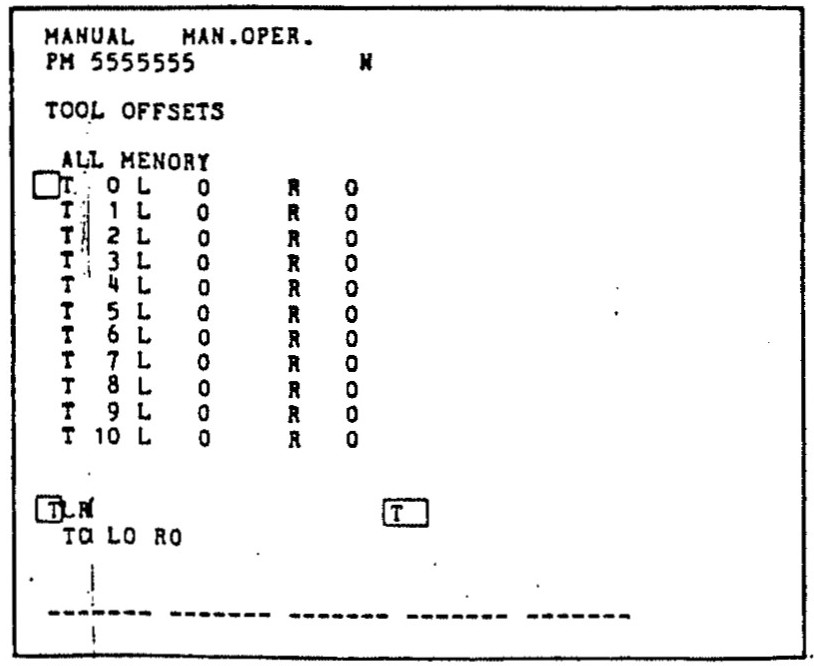
\includegraphics[width=0.7\textwidth]{tool_data_screen.jpg}
    \caption{Tool Data List Display}
\end{figure}

\newpage

\subsubsection*{First Search Method}

\begin{itemize}
    \iconitem {Move the cursor to the line with the desired tool number \textbf{T} by pressing the \textbf{up} or \textbf{down} command buttons.}{up.jpg, down.jpg}
\end{itemize}

\subsubsection*{Second Search Method}

\begin{itemize}
    \item Enter the desired tool number \textbf{T} using the numeric keyboard.
    \iconitem {Press the \textbf{ENTER} button.}{enter.jpg}
    \vspace{.6cm}
    \iconitem {Press the \textbf{SEARCH} button.}{search.jpg}
\end{itemize}

The line containing the desired tool number \textbf{T} then appears at the top of the tool data list section displayed on the screen.

The lower screen cursor is now positioned at letter-address \textbf{L}. It must be moved to letter-address \textbf{T} if the search procedure needs to continue.

\textbf{Note:} It is recommended to always use the \textbf{second method} when the desired tool number \textbf{T} is outside the currently visible tool data section on the screen.

\subsection{Entering and Modifying Tool Data}

Entering or modifying tool data under tool numbers \textbf{T1 ... T255} is only possible in \textbf{MANUAL} mode.

No entries can be made under tool number \textbf{T0}.

\procedure

\begin{itemize}
    \iconitem {Press the \textbf{MANUAL} button.}{manual.jpg}
    \vspace{.6cm}
    \iconitem {Press the \textbf{TOOL MEM} button.}{tool_mem.jpg}
    \vspace{.5cm}
    \item Search for the tool number \textbf{T} under which the tool data should be entered or modified (see Section \textbf{4.1.1}).
    \iconitem {Move the cursor to letter-address \textbf{L} by pressing the \textbf{left} or \textbf{right} command buttons.}{left.jpg, right.jpg}
    \item Enter the tool length \textbf{L} value using the numeric keyboard.
    \iconitem {Press the \textbf{ENTER} button.}{enter.jpg}
\end{itemize}

\vspace{.5cm}

After pressing the \textbf{ENTER} button, the cursor moves to letter-address \textbf{R}.

\begin{itemize}
    \item Enter the tool radius \textbf{R} value using the numeric keyboard.
    \iconitem {Press the \textbf{ENTER} button.}{enter.jpg}
\end{itemize}

\vspace{.5cm}
After correctly entering the tool data \textbf{L} and \textbf{R}:

\begin{itemize}
    \iconitem {Press the \textbf{STORE} button.}{store.jpg}
\end{itemize}

\vspace{.5cm}

Pressing the \textbf{STORE} button saves the tool data \textbf{L} and \textbf{R} for tool number \textbf{T} into the tool data memory \textbf{TM}.

\newpage

Once the tool data entry is completed and stored in memory:

\begin{itemize}
    \iconitem {Press the \textbf{MANUAL} button.}{manual.jpg}
\end{itemize}

\vspace{.5cm}

\notes

After storing the data for a tool number \textbf{T}, the cursor moves to the next tool number in the tool data list.

The lower cursor of the display screen is now positioned at letter-address \textbf{L}, allowing new tool data to be entered for the next tool following the same procedure.

If necessary, tool data modification is also possible (see previous procedure).

Entering new values automatically overwrites outdated parameters stored under tool number \textbf{T} in the tool data list, without requiring manual deletion.

For \textbf{reading and writing tool data}, refer to Sections \textbf{8.2.1} and \textbf{8.2.2}.

\subsection{Tool Data Control}

If necessary, tool data from the tool data list can be checked during program execution.

\begin{itemize}
    \iconitem {Press the \textbf{TOOL MEM} button.}{tool_mem.jpg}
\end{itemize}

Tool data can now be reviewed.

\textbf{Searching for a Tool Number T:} See Section \textbf{4.1.1}.

After checking the tool data:

\begin{itemize}
    \iconitem {Press one of the buttons: \textbf{TEACH IN}, \textbf{SINGLE}, or \textbf{AUTO}, depending on the displayed signal at line \textbf{1} of the screen.}{teach_in.jpg, single.jpg, auto.jpg}
\end{itemize}

\vspace{.5cm}

Once the corresponding button is pressed, the selected operating mode appears on the screen.

\subsection{Deleting Data for a Single Tool}

\begin{itemize}
    \iconitem {Press the \textbf{MANUAL} button.}{manual.jpg}
    \vspace{.6cm}
    \iconitem {Press the \textbf{TOOL MEM} button.}{tool_mem.jpg}
    \item Search for the tool number \textbf{T} whose data needs to be deleted (see Section \textbf{4.1.1}).
    \iconitem {Move the cursor to letter-address \textbf{T} using the left/right command buttons.}{left.jpg, right.jpg}
    \vspace{.6cm}
    \iconitem {Press the \textbf{ENTER} button.}{enter.jpg}
\end{itemize}

The tool number \textbf{T} appears with the complement \textbf{(CLEAR)} at line \textbf{21} on the screen.

\begin{itemize}
    \iconitem {Press the \textbf{STORE} button.}{store.jpg}
\end{itemize}

Pressing the \textbf{STORE} button deletes the data for a single tool. Under the selected tool number in the tool data list, the value \textbf{0} is now displayed for the tool’s length \textbf{L} and radius \textbf{R}.

If no further modifications are needed for the tool data memory:

\begin{itemize}
    \iconitem {Press the \textbf{MANUAL} button.}{manual.jpg}
\end{itemize}

\newpage

\subsection{Deleting Data for All Tools}

\begin{itemize}
    \iconitem {Press the \textbf{MANUAL} button.}{manual.jpg}
    \vspace{.6cm}
    \iconitem {Press the \textbf{TOOL MEM} button.}{tool_mem.jpg}
    \vspace{.6cm}
    \iconitem {Move the cursor to the line \textbf{ALL MEMORY} using the up/down command buttons.}{up.jpg, down.jpg}
    \vspace{.6cm}
    \iconitem {Press the \textbf{ENTER} button.}{enter.jpg}
\end{itemize}

\vspace{.5cm}
The indicator \textbf{ALL MEMORY} followed by the complement \textbf{CLEAR} appears at \textbf{line 21} on the visualization screen.

\begin{itemize}
    \iconitem{ Press the \textbf{STORE} button.}{store.jpg}
\end{itemize}

\vspace{.5cm}
Pressing the \textbf{STORE} button deletes the data for \textbf{all tools}. Under all tool numbers in the tool data list, the value \textbf{0} is now displayed for tool length \textbf{L} and tool radius \textbf{R}.

If no further data entry is required in the tool data memory:

\begin{itemize}
    \iconitem {Press the \textbf{MANUAL} button.}{manual.jpg}
\end{itemize}
\vspace{.5cm}
\notes

For machines equipped with an automatic tool changer, during each tool deletion procedure, tool position numbers \textbf{P} in the tool magazine are automatically assigned to all tool numbers \textbf{T} on the right side of the tool data list.

See also Section \textbf{4.1.6}.

\newpage

\subsection{Entering Position Numbers in Magazine P in Tool Data Memory}

For machines with an automatic tool changer, tool numbers \textbf{T} and their corresponding position numbers in the tool magazine \textbf{P} must be linked.

This assignment is recorded in the tool data list of the tool data memory \textbf{TM}. It is also shown in the tool service life list (see Section \textbf{4.2}), associated with the tool service life memory \textbf{TL}.

As long as tool data is not stored in the tool data memory, the value \textbf{0} is displayed in the tool data list for tool length \textbf{L} and tool radius \textbf{R} under all tool numbers \textbf{T}.

The position numbers in magazine \textbf{P1 ... P255} are displayed on the right side of the tool data list, below tool numbers \textbf{T1 ... T255} (specific to the machine).

An identical assignment of tool numbers \textbf{T} to position numbers in magazine \textbf{P} is always made when \textbf{all tools} are deleted (see Section \textbf{4.1.5}).

The automatic identical assignment of tool numbers \textbf{T} to position numbers in magazine \textbf{P} is only retained if all tools \textbf{T} used are mounted in magazine \textbf{P} in the same positions as when the tool magazine was originally equipped.

However, if the tools are arranged in the magazine in a different order, it is necessary to enter the actual position of the tool in magazine \textbf{P} for each tool used under its tool number \textbf{T} (\textbf{position coding variability}).

Entering position numbers in magazine \textbf{P} in tool data memory must be done following the procedure described in Section \textbf{4.1.2}.

\notes

\begin{itemize}
    \item Each position number in magazine \textbf{P} can appear only once in the tool data list.
    \item Position numbers in magazine \textbf{P} \textbf{cannot be written or read}.
\end{itemize}

\newpage

\section{Tool Life Monitoring (TOOL LIFE)}

Tool service life \textbf{C} can be stored under tool numbers \textbf{T1 ... T255} for up to \textbf{255 tools} in the tool life memory \textbf{TL}.

In this case, tool service life \textbf{C} (in minutes) are recorded in a tool life data list.

Tool service life recorded in the tool life data list are monitored by the control system.

When the monitored tool life \textbf{C} has expired, the signal \textbf{ERROR 111} is displayed on \textbf{line 3} of the screen.

The program execution continues, and the tool with the expired service life remains in service until the next tool change.

After the next introduction of tool change instruction data, the tool number \textbf{T} under which the tool life \textbf{C} has expired is \textbf{blocked} and thus removed from use.

The procedure to follow after a tool’s service life \textbf{C} has expired is detailed in Section \textbf{4.2.5}.

\subsubsection*{Monitoring Tool Service Life}

Tool service life can be checked at any time during program execution (see Section \textbf{4.2.2}).

In addition to the preset value of the tool service life \textbf{C}, the \textbf{current tool service life} \textbf{A} is displayed in the tool service life list associated with the tool service memory for tool numbers \textbf{T} where a tool service life \textbf{C} has been recorded. The value \textbf{A} represents the time already elapsed from the programmed tool service life \textbf{C}.

The \textbf{remaining tool service life} \textbf{R} of the tool is displayed in the third column of the tool service life data list.

\textbf{Note:}
\begin{itemize}
    \item For machines equipped with an automatic tool changer, the tool position number in magazine \textbf{P} is displayed on the right side of the tool service life list.
\end{itemize}

See also Section \textbf{4.1.6}.

\newpage

\subsection{Entering and Modifying Tool Service Life}

The introduction and modification of data related to the service life of tools under tool numbers \textbf{T1 ... T255} is only possible in \textbf{MANUAL} mode.

No entries can be made under tool number \textbf{T0}.

\procedure

\begin{itemize}
    \iconitem {Press the \textbf{MANUAL} button.}{manual.jpg}
    \vspace{.6cm}
    \iconitem {Press the \textbf{TOOL MEM} button.}{tool_mem.jpg}
    \vspace{.6cm}
    \iconitem {Press the \textbf{MENU} button.}{menu.jpg}
\end{itemize}

\vspace{.5cm}

The submenu for tool programming appears on the screen:

\begin{center}
    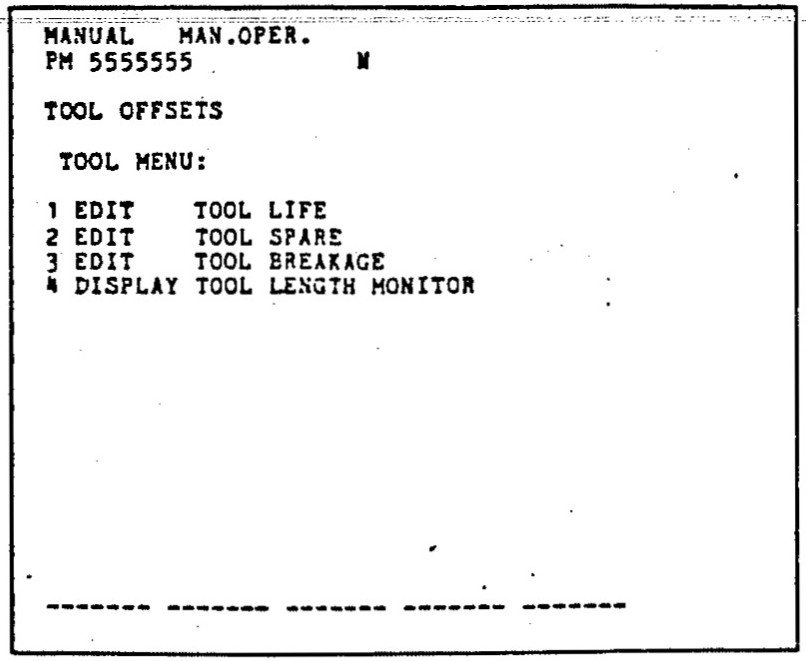
\includegraphics[width=0.7\linewidth]{tool_menu.jpg}
\end{center}

\begin{itemize}
    \iconitem {Press the \textbf{1} key on the numeric keyboard to select \textbf{EDIT TOOL LIFE}.}{one.jpg}
\end{itemize}

\newpage

The tool service life list appears on the screen:

\begin{center}
    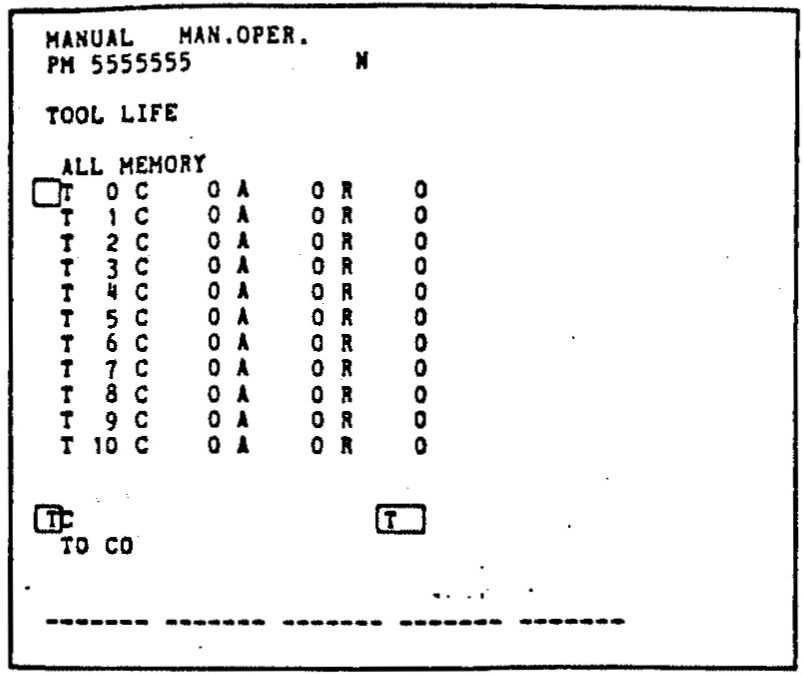
\includegraphics[width=0.7\linewidth]{tool_service_list.jpg}
\end{center}

\subsubsection*{Entering the Tool Service Life}

\begin{itemize}
    \item Search for the tool number \textbf{T} under which the tool service life value \textbf{C} needs to be entered or modified (see Section \textbf{4.1.1}).
    \iconitem {Move the cursor to the address letter \textbf{C} by pressing one of the \textbf{left-right} command buttons.}{left.jpg, right.jpg}
    \item Enter the tool service life \textbf{C} in minutes using the numeric keypad.
    \iconitem {Press the \textbf{ENTER} button.}{enter.jpg}
    \vspace{.6cm}
    \iconitem {Press the \textbf{STORE} button.}{store.jpg}
\end{itemize}
\vspace{.5cm}
The activation of the \textbf{STORE} button saves the tool service life \textbf{C} value for the selected tool number \textbf{T} in the tool service life memory \textbf{TL}.

\begin{itemize}
    \iconitem {Once the entry is complete in the tool service life memory, press the \textbf{MANUAL} button.}{manual.jpg}
\end{itemize}

\notes

If necessary, the tool service life \textbf{C} must be \textbf{modified} as described earlier.

Changing the preset service life value \textbf{C} for a tool automatically updates the remaining life \textbf{R} of that tool in the service life data list.

Before entering the service life of a new tool, the elapsed life of the previously used tool must be cleared (see section 4.2.3).

\textbf{Writing and reading the tool life}, see section 8.2.3.

\newpage

\subsection{Tool Life Monitoring}

If necessary, tool service life can be monitored from the tool service life list during program execution.

\begin{itemize}
    \iconitem {Press the \textbf{TOOL MEM} key and the \textbf{MENU} key.}{tool_mem.jpg,menu.jpg}
    \vspace{.5cm}
    \item The submenu for tool programming appears on the screen.
    \item Press \textbf{1} on the numeric keypad to select \textbf{DISPLAY TOOL LIFE}.
\end{itemize}

The tool life can now be monitored.

\textbf{Searching for a tool number T}, see section 4.1.1.

Once the tool life monitoring is completed:

\begin{itemize}
    \iconitem {Press the \textbf{TEACH IN}, \textbf{SINGLE}, or \textbf{AUTO} key according to the indication displayed on line 1 of the visualization screen (\textbf{TEACH IN}, \textbf{SINGLE}, or \textbf{AUTO}).}{teach_in.jpg,single.jpg,auto.jpg}
    \item Pressing the appropriate key will display the selected operating mode on the screen.
\end{itemize}

\subsection{Erasing the Tool Service Life of a Single Tool}

Select the operating sub-mode \textbf{EDIT TOOL LIFE} (see section 4.2.1), then:

\begin{itemize}
    \item Search for the tool number \textbf{T} under which the tool service life of tool \textbf{C} must be erased (see section 4.1.1).
\end{itemize}

\begin{itemize}
    \iconitem{Move the cursor to the letter-address \textbf{T} by pressing the left and right command keys.}{left.jpg,right.jpg}
\end{itemize}

% \marginnoteicon{5.7cm}{enter.jpg}

\begin{itemize}
    \iconitem{Press the \textbf{ENTER} key.}{enter.jpg}
\end{itemize}

The selected tool number \textbf{T}, followed by the complement \textbf{CLEAR}, is displayed on line 21 of the screen.

\begin{itemize}
    \iconitem{Press the \textbf{STORE} key.}{store.jpg}
\end{itemize}

Pressing the \textbf{STORE} key erases the tool service life of the selected tool.  
The value \textbf{0} is then displayed in the tool service life data list under the selected tool number for:  
- The preset tool service life \textbf{C},  
- The current tool service life \textbf{A},  
- The remaining tool service life \textbf{R}.

If no further modifications should be made to the tool service life memory:

\marginnoteicon{11.0cm}{}
\begin{itemize}
    \iconitem{Press the \textbf{MANUAL} key.}{manual.jpg}
\end{itemize}

\newpage

\subsection{Erasing the Tool Service Life of All Tools}

Select the operating sub-mode \textbf{EDIT TOOL LIFE} (see section 4.2.1), then:

\begin{itemize}
    \iconitem{Move the cursor to the line \textbf{ALL MEMORY} by pressing the up and down command keys.}{up.jpg,down.jpg}
\end{itemize}
\vspace{.5cm}
\begin{itemize}
    \iconitem{Press the \textbf{ENTER} key.}{enter.jpg}
\end{itemize}
\vspace{.5cm}
\begin{itemize}
    \item The indication \textbf{ALL MEMORY}, followed by the complement \textbf{CLEAR}, is displayed on line 21 of the screen.

    \iconitem{Press the \textbf{STORE} key.}{store.jpg}
\end{itemize}

\vspace{.5cm}

Pressing the \textbf{STORE} key erases the tool service life of \textbf{all tools}.  
The value \textbf{0} is then displayed in the tool service life data list under all tool numbers for:  

\begin{itemize}
    \item The preset tool service life \textbf{C}
    \item The current tool service life \textbf{A}
    \item The remaining tool service life \textbf{R}
\end{itemize}


If no further entries should be made in the tool service life memory after the erasure procedure:

\begin{itemize}
    \iconitem{Press the \textbf{MANUAL} key.}{manual.jpg}
\end{itemize}

\newpage

\subsection{Tool Release at the End of Tool Service Life}

The tool service life monitoring system releases tool numbers \textbf{T} for which the tool service life has expired in the tool service life list. The affected tool is then removed from use for machining the workpiece.

\textbf{Monitoring the Tool Service Life}, see section 4.2.

Tool numbers \textbf{T} that are blocked must be \textbf{released} again:

\begin{itemize}
    \item To allow the use of a new tool with the same tool number \textbf{T} after clearing the expired tool service life \textbf{C} of the previous tool and entering the new tool service life for machining.
    
    \item To allow the reuse of the previous tool after its tool service life has expired, following an extension of tool service life \textbf{C} for machining.
\end{itemize}

The tool release must be performed in the memory of replacement tools \textbf{TS}. The procedure is described at the end of this section.

\textbf{Replacement Tools}, see section 4.3.

\vspace{.5cm}

\textbf{Machines Without an Automatic Tool Changer}

\begin{itemize}
    \item The indicator \textbf{ERROR I11} alerts the operator that the previous tool, whose tool service life has expired, must no longer be used and that a new tool must be made available.

    \item The indicator \textbf{ERROR I11} may be cleared as soon as the first instruction to change the tool has been executed after its display on the screen.

    \item It is advisable to clear the \textbf{ERROR I11} indicator only after the new tool has been made available and its data has been entered.
\end{itemize}

If \textbf{no replacement tool} is determined in the memory of replacement tools for a blocked tool number, the blocked tool number must be released before selecting a tool with the same number.

Before doing so, the expired tool service life must be erased (see section 4.2.3) and re-entered into the tool service life memory (see section 4.2.3) under the blocked tool number.

If a replacement tool is determined in the memory of replacement tools for a blocked tool number, the indication \textbf{INTERVENTION T}, followed by the number of the replacement tool, appears on line 2 of the screen when the blocked tool number is next called.

The operator must then insert the prepared replacement tool with the tool number \textbf{T} \textbf{displayed} on the screen into the spindle of the machine.

Before the tool service life \textbf{C} of the replacement tool expires, the number of the original blocked tool must be \textbf{released} again.

Before doing so, the expired tool service life must be erased (see section 4.2.3) and re-entered into the tool service life memory (see section 4.2.1) under the blocked tool number.

Additionally, after being made available, the data of the new original tool must be entered.

\newpage

\textbf{Machines with an Automatic Tool Changer}

\begin{itemize}
    \item The indicator \textbf{ERROR I11} alerts the operator that the previous tool, whose tool service life has expired, must be removed from the tool magazine and replaced with a new tool.

    \item It is advisable to clear the \textbf{ERROR I11} indicator only after the new original tool has been placed in the tool magazine.

    \item Calling a tool number that is blocked because its tool service life \textbf{C} has expired will display the indication \textbf{INTERVENTION T}, followed by the number of the replacement tool, on line 3 of the screen.
    
    \item The replacement tool is changed automatically.

    \item Before the tool service life \textbf{C} of the replacement tool expires, the number of the original tool must be \textbf{released} again.

    \item Before doing so, the expired tool service life must be erased (see section 4.2.3) and re-entered into the tool service life memory (see section 4.2.1) under the blocked tool number.

    \item Additionally, the tool data must be entered after making a new original tool available.
\end{itemize}

\newpage

\subsection{Releasing a Blocked Tool Number \textbf{T}}

\begin{itemize}
    \iconitem{Press the \textbf{MANUAL} key.}{manual.jpg}
    \vspace{.6cm}
    \iconitem{Press the \textbf{TOOL MEM} key.}{tool_mem.jpg}
    \vspace{.6cm}
    \iconitem{Press the \textbf{MENU} key.}{menu.jpg}
\end{itemize}

\vspace{.5cm}

The submenu for tool programming appears on the screen:

\begin{center}
    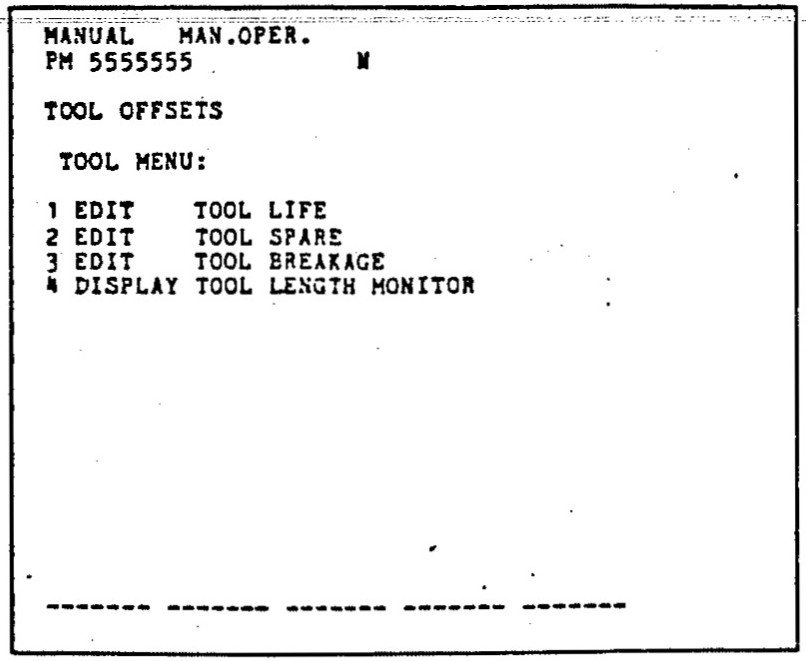
\includegraphics[width=0.6\textwidth]{tool_menu.jpg}
\end{center}

\begin{itemize}
    \item Press \textbf{2} on the numeric keypad to select \textbf{EDIT TOOL SPARE}.
    \iconitem{Move the cursor to the blocked tool number \textbf{T} by pressing the up and down command keys.}{up.jpg,down.jpg}
\end{itemize}

The letter-address \textbf{T} of a blocked tool number is displayed on the screen in \textbf{inverted} format.

\begin{itemize}
    \item Enter the \textbf{number} of the tool to be released without the equal sign on the numeric keypad.
    \iconitem{Press the \textbf{ENTER} key.}{enter.jpg}
    \vspace{.6cm}
    \iconitem{Press the \textbf{F2} function key.}{f2.jpg}
\end{itemize}

After pressing the \textbf{F2} key, the blocked tool number is released again and can be used for machining.

If no further modifications should be made to the memory of replacement tools:

\begin{itemize}
    \iconitem{Press the \textbf{MANUAL} key.}{manual.jpg}
\end{itemize}
\vspace{.5cm}
\notes

Replacement tool numbers should not be used within the machining program.

For a tool number \textbf{T} activated with function \textbf{M67}, a tool service life \textbf{C} must not be indicated in the tool service life list.

\begin{itemize}
    \item If a tool has been released unintentionally, it is possible to lock it again by following the procedure described above and pressing the \textbf{F1} function key.
\end{itemize}

\newpage

\section{Spare Tools}

A \textbf{spare tool} is a replacement tool for the original tool. Both tools serve the same purpose; however, they differ in terms of the actual tool data values (length \textbf{L} and radius \textbf{R}).

A spare or replacement tool is used when the original tool is blocked from further machining (e.g., due to the expiration of the service life of the monitored tool).

\textbf{Monitoring the Tool Service Life}, see section 4.2.

A spare tool can be assigned to each original tool.  
This assignment is made in the list of tool numbers stored in the \textbf{IS} spare tool memory.

If a tool number \textbf{T1 ... T255} in the \textbf{right column} is assigned to a tool number \textbf{T1 ... T255} listed in the \textbf{left column}, the tool number in the right column becomes the spare tool number.  
This tool number is automatically removed from the left column of the list and can no longer be used in the machining program.

Only the original tool numbers from the left column of the spare tool list can be used in the machining program.  
All tool numbers in the right column are spare tool numbers.

The tool data of the spare tool in the spare tool list memory \textbf{TM} must be recorded under tool number \textbf{T} of the spare tool.

\textbf{Tool Data}, see section 4.1.

The service life \textbf{C} of the spare tool must be recorded in the tool service life list of the tool service life memory \textbf{TL} under tool number \textbf{T} of the spare tool.

\textbf{Entering the Tool Service Life}, see section 4.2.1.

For machines \textbf{with an automatic tool changer}, it is necessary that spare tools are also available in the tool magazines.  
If the total number of tools used exceeds the number of magazine slots \textbf{P}, manual tool changes must be performed.

Both tools (the original tool and the spare tool) must be changed automatically using function \textbf{M66}.  
After the original tool has been automatically changed (function \textbf{M6}), the spare tool \textbf{cannot be changed manually} (function \textbf{M66}).

\newpage

\subsection{Entering and Modifying Spare Tools}

Spare tools can only be entered or modified in \textbf{MANUAL} mode.

\procedure

\begin{itemize}
    \iconitem{Press the \textbf{MANUAL} key.}{manual.jpg}
    \vspace{.6cm}
    \iconitem{Press the \textbf{TOOL MEM} key.}{tool_mem.jpg}
    \vspace{.6cm}
    \iconitem{Press the \textbf{MENU} key.}{menu.jpg}
\end{itemize}
\vspace{.5cm}

The submenu for tool programming appears on the screen:

\begin{center}
    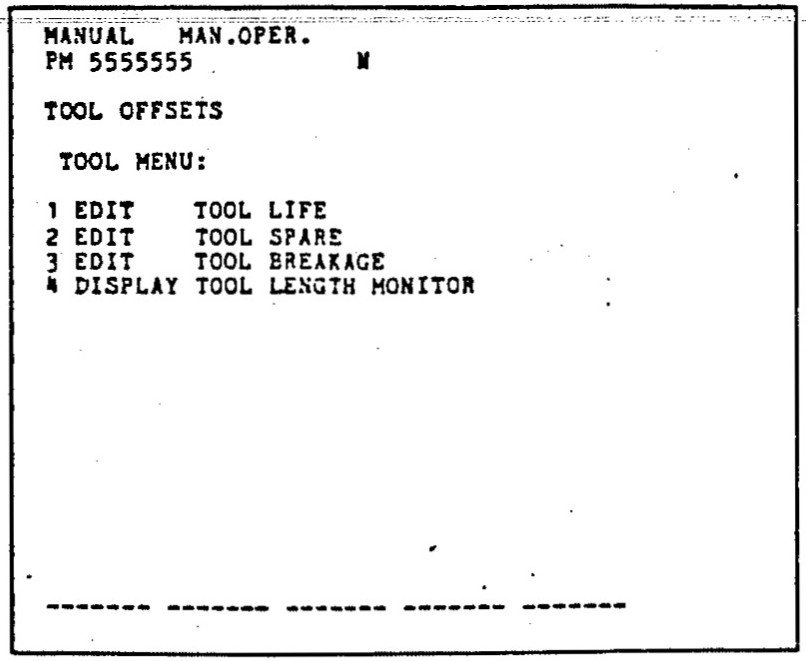
\includegraphics[width=0.7\textwidth]{tool_menu.jpg}
\end{center}

\begin{itemize}
    \item Press \textbf{2} on the numeric keypad to select \textbf{EDIT TOOL SPARE}.
\end{itemize}

\newpage

The list of tool numbers in the spare tool memory \textbf{TS} is displayed on the screen:

\begin{center}
    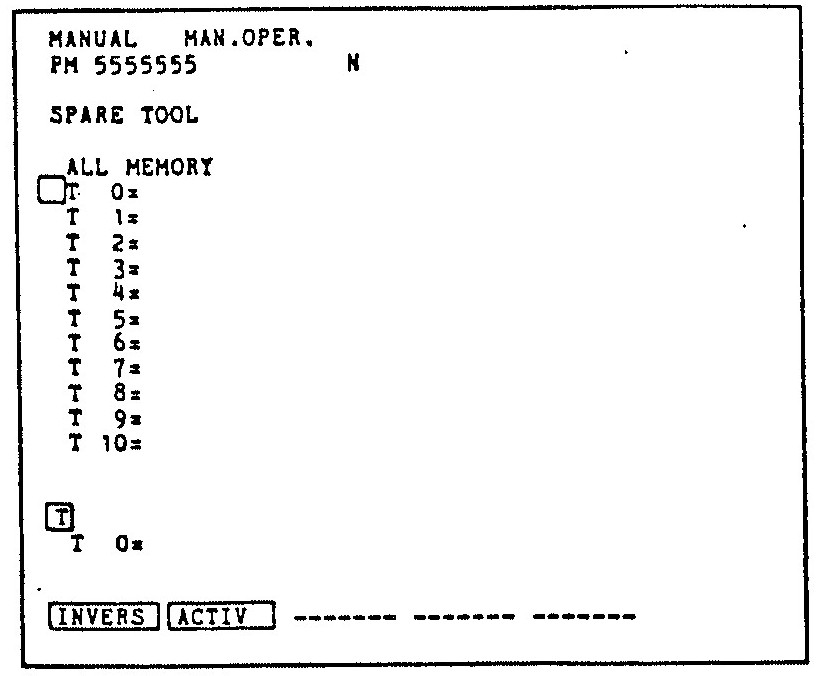
\includegraphics[width=0.7\textwidth]{spare_tool_list.jpg}
\end{center}

\vspace{.5cm}

\begin{itemize}
    \item Search for the tool number \textbf{T} under which the spare tool should be entered or modified (see section 4.1.1).
    \item Enter the found tool number using the numeric keypad.
    \iconitem{Press the \textbf{EQUAL} key.}{equal.jpg}
    \vspace{.6cm}
    \iconitem{Move the cursor to the letter-address \textbf{T} by pressing the left and right command keys.}{left.jpg,right.jpg}
    \item Enter the spare tool number using the numeric keypad.
    \iconitem{Press the \textbf{ENTER} key.}{enter.jpg}
    \vspace{.6cm}
    \iconitem{Press the \textbf{STORE} key.}{store.jpg}
\end{itemize}

\vspace{.5cm}
Pressing the \textbf{STORE} key saves the spare tool in the spare tool memory \textbf{TS}.

The spare tool number, now listed in the right column of the tool number list under the selected tool number, no longer appears in the left column and must not be used in the program.

Once the spare tool data entry is complete:

\begin{itemize}
    \iconitem{Press the \textbf{MANUAL} key.}{manual.jpg}
\end{itemize}

\vspace{.5cm}
\notes

If necessary, it may also be required to \textbf{modify} the spare tools as previously described.

No entry is possible under tool number \textbf{T0}.

\textbf{Writing and Reading Spare Tools}, see section 8.2.4.

\subsection{Spare Tool Monitoring}

If necessary, the spare tools from the spare tool list can be monitored during program execution.

\begin{itemize}
    \iconitem{Press the \textbf{TOOL MEM} key and the \textbf{MENU} key.}{tool_mem.jpg,menu.jpg}
\end{itemize}

The submenu for tool programming appears on the screen.

\begin{itemize}
    \item Enter \textbf{2} by pressing the numeric keypad to select \textbf{DISPLAY TOOL SPARE}.
\end{itemize}

The spare tools can now be monitored.

\textbf{Searching for a Tool Number T}, see section 4.1.1.

Once the spare tool monitoring is complete:

\begin{itemize}
    \iconitem{Press the \textbf{TEACH IN}, \textbf{SINGLE}, or \textbf{AUTO} key according to the indication displayed on line 1 of the screen (\textbf{TEACH IN}, \textbf{SINGLE}, or \textbf{AUTO}).}{teach_in.jpg,single.jpg,auto.jpg}
\end{itemize}

Pressing the appropriate key will display the selected operating mode on the screen again.

\subsection{Erasing a Single Spare Tool}

After selecting the sub-mode \textbf{EDIT TOOL SPARE} (see section 4.3.1):

\begin{itemize}
    \item Search for the tool number \textbf{T} under which the spare tool should be erased (see section 4.1.1).
    \item Enter the found tool number using the numeric keypad.
    \iconitem{Press the \textbf{EQUAL} key.}{equal.jpg}
    \vspace{.6cm}
    \iconitem{Press the \textbf{ENTER} key.}{enter.jpg}
    \vspace{.6cm}
    \iconitem{Press the \textbf{STORE} key.}{store.jpg}
\end{itemize}

Pressing the \textbf{STORE} key deletes the \textbf{individual spare tool} from the spare tool memory \textbf{TS}.

The deleted spare tool number is now included in the left column of the tool number list as the original tool number and can once again be used in the program.

If no further modifications should be made to the spare tool memory:

\begin{itemize}
    \iconitem{Press the \textbf{MANUAL} key.}{manual.jpg}
\end{itemize}


\newpage
\subsection{Erasing All Spare Tools}

After selecting the sub-mode \textbf{EDIT TOOL SPARE} (see section 4.3.1):

\begin{itemize}
    \iconitem{Move the cursor to the line \textbf{ALL MEMORY} by pressing the up and down command keys.}{up.jpg,down.jpg}
    \iconitem{Press the \textbf{ENTER} key.}{enter.jpg}
\end{itemize}
\vspace{.5cm}

The indication \textbf{ALL MEMORY}, followed by the complement \textbf{CLEAR}, is displayed on line 21 of the screen.

\begin{itemize}
    \iconitem{Press the \textbf{STORE} key.}{store.jpg}
\end{itemize}
\vspace{.5cm}

Pressing the \textbf{STORE} key erases \textbf{all} spare tools in the spare tool memory \textbf{TS}.

The deleted spare tool numbers are now included in the left column of the tool number list as original tool numbers and can once again be used in the program.

If, after erasure, no further entries should be made in the spare tool memory:

\begin{itemize}
    \iconitem{Press the \textbf{MANUAL} key.}{manual.jpg}
\end{itemize}
